\subsection{Silencing the Charge: Tips for Quieter Battery Boosting!}

\begin{tcolorbox}[colback=gray!10, colframe=black, title=E4E04] How can conducted noise from an automobile battery charging system be suppressed?  
\begin{enumerate}[label=\Alph*.]
    \item By installing filter capacitors in series with the alternator leads
    \item By installing a noise suppression resistor and a blocking capacitor at the battery
    \item By installing a high-pass filter in series with the radio’s power lead and a low-pass filter in parallel with the antenna feed line
    \item \textbf{By installing ferrite chokes on the charging system leads}
\end{enumerate} \end{tcolorbox}

\subsubsection{Related Concepts}

Conducted noise in automobile electronic systems is often a result of electromagnetic interference (EMI) generated by various electrical components during operation, particularly the charging system. In the context of this question, we specifically consider noise that affects radio communications due to its potential to disrupt signals and audio clarity.

Ferrite chokes are passive components that use ferrite materials to suppress high-frequency noise. They act as inductors at high frequencies, presenting a high impedance to unwanted noise while allowing the desired DC or lower-frequency signals to pass. This characteristic makes them particularly effective for suppressing conducted noise generated by components like alternators, which can introduce noise into the vehicle's electrical system.

In contrast, installing filter capacitors or noise suppression resistors might not effectively address the high-frequency noise. While these components can improve power supply regulation, they do not have the same level of effectiveness against high-frequency radiated noise as ferrite chokes do.

To better understand the concept, consider the following basic principles:

1. \textbf{Conducted vs. Radiated Noise}: Conducted noise affects the power lines and can travel through the electrical connections, whereas radiated noise is emitted into the air and can affect radio wave propagation.
   
2. \textbf{Impedance and Filtering}: High-frequency noise can be viewed as a signal that sees a high impedance (inductor behavior) on the path to ground or other sensitive connections (like the radio).

\subsubsection{Calculation Example}

For the calculation aspect, consider the effectiveness of using ferrite chokes. Let's say the ferrite choke has an impedance \( Z \) expressed as:

\[
Z = j\omega L \quad \text{where} \quad \omega = 2\pi f
\]

- Let \( L = 10 \, \text{mH} \) (millihenries) and analyze at a frequency \( f = 100 \, \text{kHz} \).
  
Calculating the angular frequency:

\[
\omega = 2\pi f = 2\pi \times 100,000 \approx 628,318
\]

Calculating \( Z \):

\[
Z = j(628318)(0.01) \approx j6283.18 \, \Omega
\]

This indicates that at 100 kHz, the choke presents a significant impedance to the high-frequency noise, effectively filtering it out.

\subsubsection{Illustrative Diagram}

Below is a TikZ diagram illustrating the placement of ferrite chokes in the automobile charging system:

\begin{center}
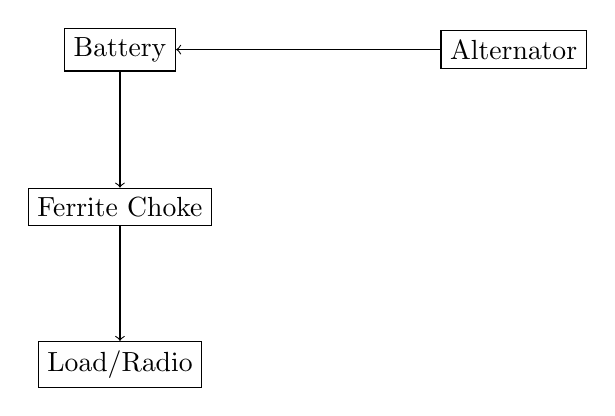
\begin{tikzpicture}[node distance=2cm]
    \node (battery) [draw, rectangle] {Battery};
    \node (ferrite) [draw, rectangle, below of=battery] {Ferrite Choke};
    \node (alternator) [draw, rectangle, right of=battery, xshift=3cm] {Alternator};
    \node (load) [draw, rectangle, below of=ferrite] {Load/Radio};

    \draw[->] (battery) -- (ferrite);
    \draw[->] (ferrite) -- (load);
    \draw[->] (alternator) -- (battery);
\end{tikzpicture}
\end{center}

In the diagram, the ferrite choke is placed between the battery and the load (e.g., the radio) to minimize the conducted noise from the alternator, effectively contributing to a clearer communication signal while charging.